\section{Sobre o projeto}

A solução apresentada foi desenvolvida em um repositório do Github chamado ``filipecancio/sbc-template'' (figura~\ref{fig:fig10}) possuindo o template LaTex oficial da SBC (Sociedade Brasileira de Computação) para a produção de artigos. O acesso está disponível em ``https://github.com/filipecancio/artigo-final''. O repositório, ao ser acessado, se converte em um ambiente de desenvolvimento (Devcontainer), aonde não há necessidade de conhecimento em programação, basta editar qualquer arquivo ``.tex'' e é gerado um ``.pdf'' formatado no padrão SBC.

\begin{figure}[ht]
	\centering
	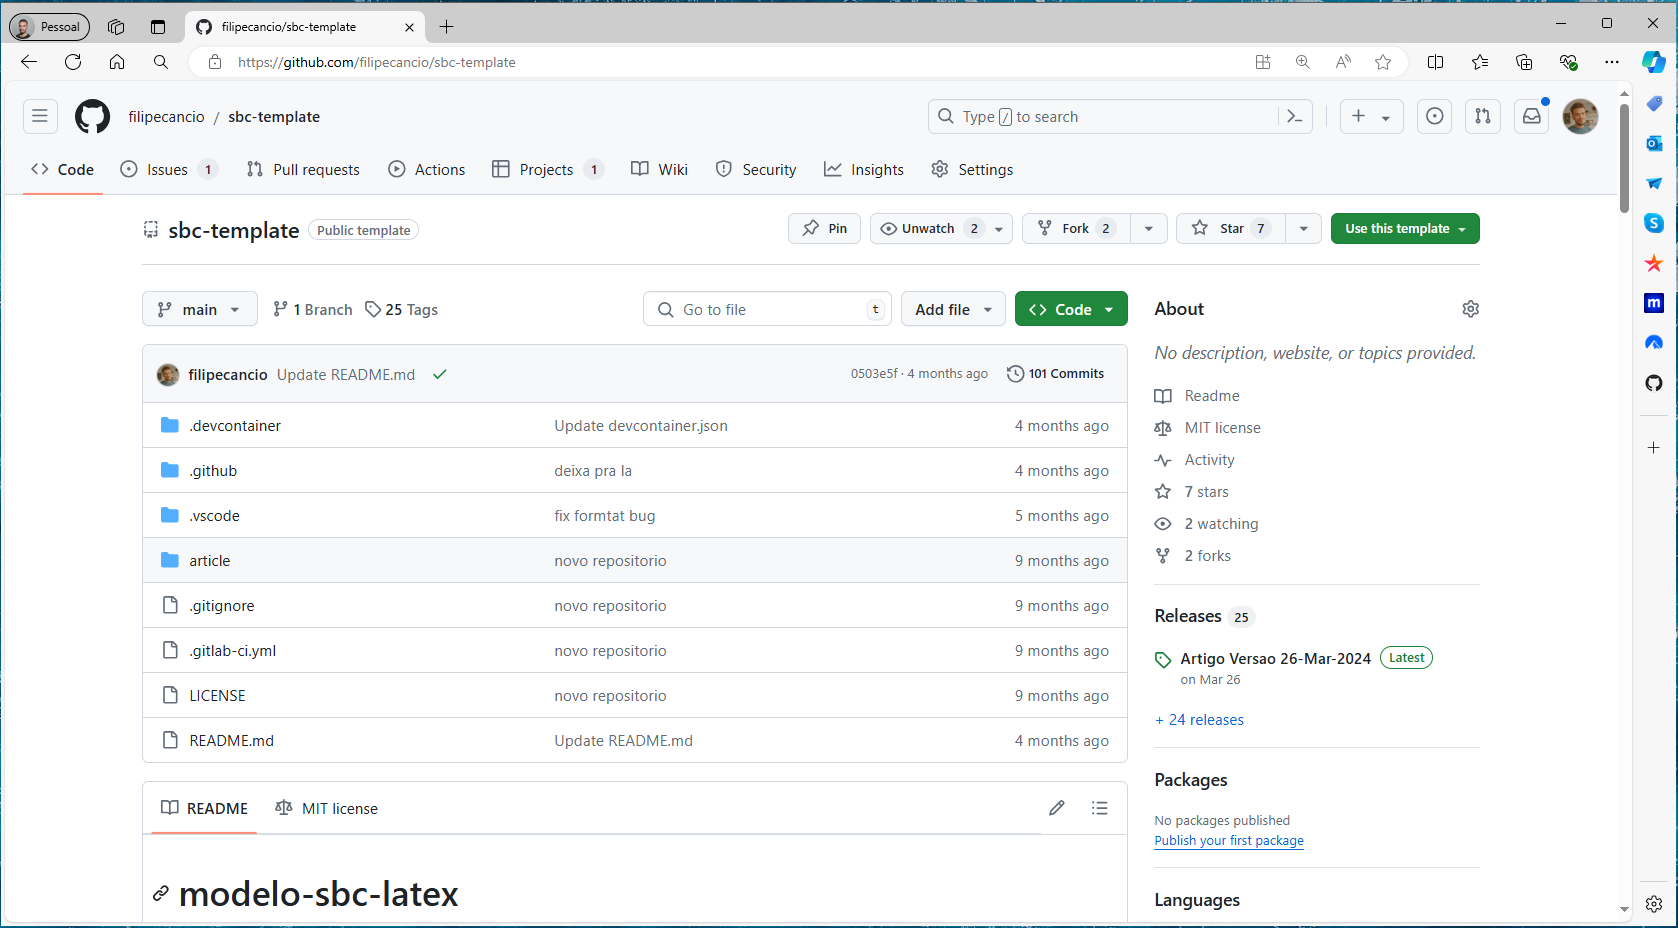
\includegraphics[width=.7\textwidth]{./images/fig10.png}
	\caption{repositorio sbc-template}
	\label{fig:fig10}
\end{figure}

\subsection{Funcionalidades}

Como solução alternativa às plataformas apresentadas abaixo (ver tabela~\ref{tab:tabela01}), o projeto possui algumas funcionalidades semelhantes porém mais abrangentes e disponíveis de forma gratuita. Entre elas podemos destacar:

\begin{table}[ht]
	\centering
	\begin{tabular}{|c|c|c|c|c|}
		\hline
		Plataformas & Usa LaTex & Colaborativo & Controle de versão & Offline
		\\
		\hline
		Overleaf & Sim & Só na versao paga & Só na versao paga & Não \\
		\hline
		Microsoft Word & Não & Sim & Limitado & Sim \\
		\hline
		Google Documentos & Não & Sim & Limitado & Não \\
		\hline
		filipecancio/sbc-template & Sim & Sim & Sim & Sim \\
		\hline
	\end{tabular}
	\caption{Comparativos entre plataformas Overleaf, Word e Documentos}
	\label{tab:tabela01}
\end{table}

\begin{itemize}
	\item Colaborativo: Utiliza 100\% de ferramentas do github para escrever artigos com orientadores e outros autores.
	\item Simples mas completo: Basta clonar e editar os textos. Com um conhecimento básico de LaTex que o próprio repositório fornecem nas instruções iniciais já é possível escrever um artigo completo, mas é util também para pessoas com o conhecimento avançado em LaTex.
	\item Online e Offline: Você pode utilizar o navegador para editar, mas é possivel acessar de forma offline também.
\end{itemize}


As edições podem ocorrer de três formas: diretamente no site do GitHub (figura~\ref{fig:fig01}), pela plataforma codespaces (figura~\ref{fig:fig02}), ou de forma offline pelo Visual Studio Code (figura~\ref{fig:fig03}).


\begin{figure}[ht]
	\centering
	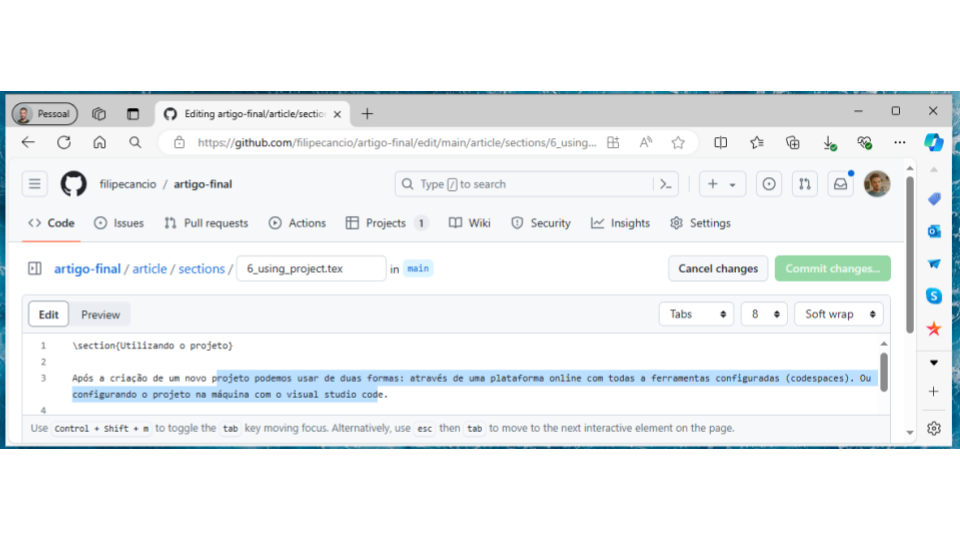
\includegraphics[width=.8\textwidth]{./images/fig03.png}
	\caption{Utilizando o projeto no site do GitHub}
	\label{fig:fig01}
\end{figure}

\begin{figure}[ht]
	\centering
	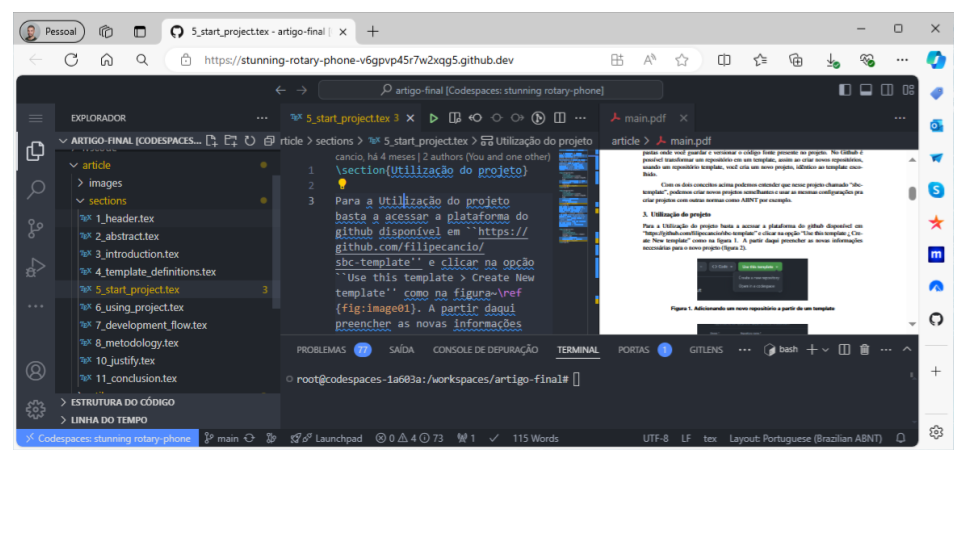
\includegraphics[width=.8\textwidth]{./images/fig02.png}
	\caption{Utilizando o projeto pelo Codespaces}
	\label{fig:fig02}
\end{figure}

\begin{figure}[ht]
	\centering
	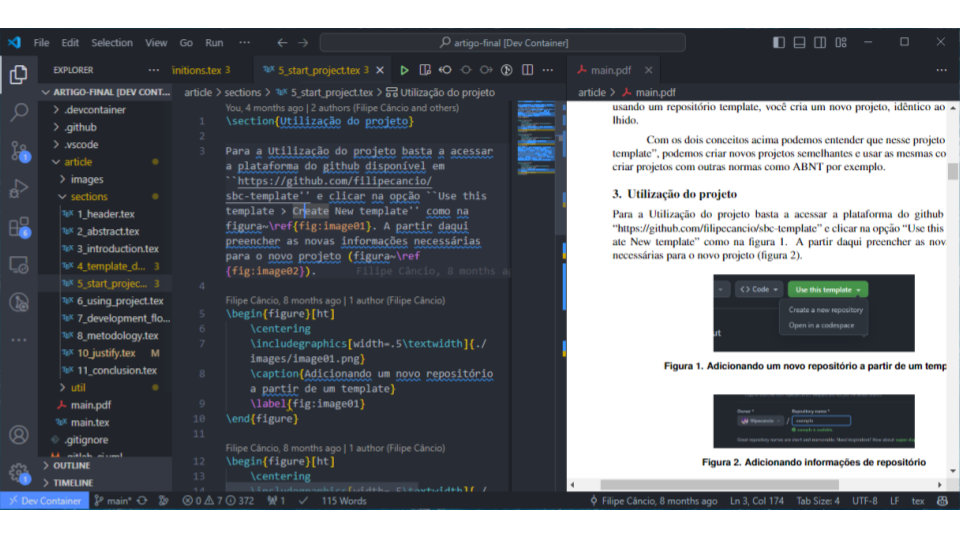
\includegraphics[width=.8\textwidth]{./images/fig01.png}
	\caption{Utilizando o projeto com Visual Studio Code}
	\label{fig:fig03}
\end{figure}

\clearpage